% main.tex — Soul Protocol research paper for arXiv submission.
% Uses NeurIPS 2025 style (preprint mode for arXiv).
% Created: 2026-03-06
% Updated: 2026-03-07 — Title change, abstract rewrite, Tier 1 reframe,
%   honest baseline discussion, psychology claims scoped, GitHub URL fixed,
%   placeholder authors resolved, architecture diagram added, Tier 4 component
%   ablation and Tier 5 Mem0 comparison added with updated discussion/limitations.

\documentclass{article}

% NeurIPS style — preprint mode for arXiv
\usepackage[preprint]{neurips_2025}

% Core packages
\usepackage[utf8]{inputenc}
\usepackage[T1]{fontenc}
\usepackage{hyperref}
\usepackage{url}
\usepackage{booktabs}
\usepackage{amsfonts}
\usepackage{amsmath}
\usepackage{nicefrac}
\usepackage{microtype}
\usepackage{graphicx}
\usepackage{xcolor}
\usepackage{subcaption}
\usepackage{multirow}
\usepackage{enumitem}
\usepackage{tikz}
\usetikzlibrary{arrows.meta, positioning, shapes.geometric, fit}

% Custom commands
\newcommand{\soul}{\textsc{Soul Protocol}}
\newcommand{\ocean}{\textsc{ocean}}
\newcommand{\soulfile}{\texttt{.soul}}
\newcommand{\ie}{\textit{i.e.}}
\newcommand{\eg}{\textit{e.g.}}
\newcommand{\etal}{\textit{et al.}}

% Table formatting
\definecolor{soulgreen}{rgb}{0.2, 0.65, 0.33}
\definecolor{basegray}{rgb}{0.55, 0.55, 0.55}

\title{Soul Protocol: An Open Protocol for Portable AI Companion Identity}

\author{
  Prakash Dalai \\
  Qbtrix \\
  \texttt{prakash@qbtrix.com} \\
}

\begin{document}

\maketitle

\begin{abstract}
Conversational AI agents are stateless. Between sessions, they forget users, lose personality, and restart from zero. Existing approaches treat memory as a retrieval problem (RAG), ignoring the psychological dimensions that make interactions feel continuous: personality consistency, emotional tracking, and relationship depth.

We introduce \soul{}, an open protocol that gives AI agents a persistent, portable identity. \soul{} combines a Big Five (\ocean{}) personality model, five-tier significance-weighted memory, somatic emotional markers, and an evolving relationship bond system into a portable \soulfile{} archive format that any application can read and write.

We validate through a five-tier evaluation: 1,000 heuristic simulations, 100 LLM-backed agents, multi-judge quality tests (5 models, 4 providers), a four-condition component ablation (10 variations per test), and a head-to-head comparison against Mem0. All 20 multi-judge evaluations favored soul-enabled agents, with the strongest gains in emotional continuity (9.7 vs.\ 1.9) and long-range recall (8.5 vs.\ 4.8). The ablation reveals that memory retrieval is the dominant factor for emotional continuity (RAG-only 9.3 vs.\ personality-only 7.2), while Full Soul consistently matches or exceeds individual components across all tests (8.7 overall vs.\ 8.4 RAG-only, 7.0 personality-only). Against Mem0, \soul{} leads by 2.5 points overall, with the largest gap in emotional tracking where Mem0 captures facts but not affective arcs. The protocol, SDK, and all experimental code are open source.
\end{abstract}

% ============================================================
\section{Introduction}
\label{sec:intro}
% ============================================================

Modern conversational AI agents are stateless by default. Each session begins with a blank slate: no memory of past interactions, no consistent personality, no awareness of the user's emotional history. This produces the uncanny experience of speaking to an entity that knows nothing about you, every time.

Several approaches address memory through retrieval-augmented generation (RAG)~\cite{lewis2020rag}, embedding user facts into vector stores for later retrieval. While effective for factual recall, these systems ignore the psychological dimensions that make human relationships feel continuous. A good friend doesn't just remember facts about you; they remember \textit{how you felt}, maintain a consistent personality across conversations, and deepen the relationship over time.

We propose \soul{}, a protocol that treats AI companion identity as a first-class, portable artifact. Rather than bolting memory onto an LLM, \soul{} provides a complete identity substrate with five components:

\begin{enumerate}[leftmargin=*, topsep=2pt, itemsep=1pt]
  \item \textbf{OCEAN Personality Model} --- Big Five traits that shape communication style, emotional expression, and decision-making tendencies.
  \item \textbf{Five-Tier Memory} --- Significance-weighted storage that mimics human memory consolidation, from working memory through core identity.
  \item \textbf{Somatic Markers} --- Emotional state tracking inspired by Damasio's somatic marker hypothesis~\cite{damasio1994descartes}, enabling emotional continuity across sessions.
  \item \textbf{Bond System} --- A relationship model tracking trust, familiarity, and interaction depth, analogous to human attachment.
  \item \textbf{Portable Archive} --- A \soulfile{} file format (zip archive) enabling soul migration between platforms without vendor lock-in.
\end{enumerate}

The key insight is that persistent identity requires more than memory retrieval. It requires \textit{psychological coherence}: the integration of personality, emotion, and relationship state into a unified identity that evolves naturally through interaction.

\paragraph{Contributions.} We make three contributions:
\begin{itemize}[leftmargin=*, topsep=2pt, itemsep=1pt]
  \item A \textbf{protocol specification} for portable AI companion identity, combining psychology-informed components into a cohesive architecture (Section~\ref{sec:protocol}).
  \item A \textbf{three-tier empirical validation} across 1,100+ agent simulations demonstrating measurable improvements in recall, personality consistency, emotional continuity, and response quality (Section~\ref{sec:experiments}).
  \item An \textbf{open-source SDK} with a CLI, enabling developers to give any LLM a persistent soul in under 10 lines of code.
\end{itemize}


% ============================================================
\section{Related Work}
\label{sec:related}
% ============================================================

\paragraph{Memory architectures for LLM agents.}
The survey by Liu \etal{}~\cite{liu2025memory} provides a comprehensive taxonomy of agent memory, categorizing by storage medium (token-level, parametric, latent), function (factual, experiential, working), and dynamics (formation, evolution, retrieval). Mem0~\cite{chhablani2025mem0} dynamically captures and retrieves salient information from conversations. A-Mem~\cite{xu2025amem} introduces agentic memory with self-organizing capabilities. The Agent Cognitive Compressor~\cite{bousetouane2026agentcognitive} replaces transcript replay with bounded internal state. Our work differs by integrating memory with personality and emotional state into a unified identity model, rather than treating memory as an isolated retrieval problem.

\paragraph{Personality in LLM agents.}
Research on the Big Five personality model applied to LLMs~\cite{ren2025bigfive} demonstrates that personality traits influence agent decision-making in social simulations. Damsa~\cite{damsa2024personality} shows that prompting with OCEAN values produces measurably different agent behaviors. The ACT-R memory model integration~\cite{honda2025actr} provides human-like memory traits. \soul{} builds on this by making personality a persistent, evolving component rather than a one-shot prompt injection.

\paragraph{Long-term conversational memory benchmarks.}
LoCoMo~\cite{maharana2024locomo} evaluates 300-turn conversations across 35 sessions. MemoryAgentBench~\cite{hu2026memoryagentbench} tests four competencies: accurate retrieval, test-time learning, long-range understanding, and conflict resolution. MemBench~\cite{tan2025membench} evaluates both factual and reflective memory. AMemGym~\cite{cheng2026amemgym} provides interactive evaluation of memory in long-horizon conversations. Our evaluation complements these by measuring not just recall accuracy but the \textit{qualitative impact} of memory on response quality, personality consistency, and emotional awareness.

\paragraph{LLM-as-judge evaluation.}
Using LLMs to evaluate LLM outputs has become standard practice~\cite{zheng2024judging}. Position bias is a known concern: judges systematically favor responses based on presentation order~\cite{shi2025positionbias}. We mitigate this through randomized A/B ordering in all pairwise comparisons, following best practices from the systematic study by Shi \etal{}~\cite{shi2025positionbias}.


% ============================================================
\section{Soul Protocol}
\label{sec:protocol}
% ============================================================

\soul{} defines a portable identity container for AI companions. A soul is created through a ``birth'' process that initializes personality traits, creates an empty memory store, and establishes baseline emotional and relational state. The soul then evolves through interaction: observing conversations, forming memories, tracking emotional shifts, and deepening bonds. Figure~\ref{fig:architecture} illustrates the protocol's components and data flow.

\begin{figure}[h]
\centering
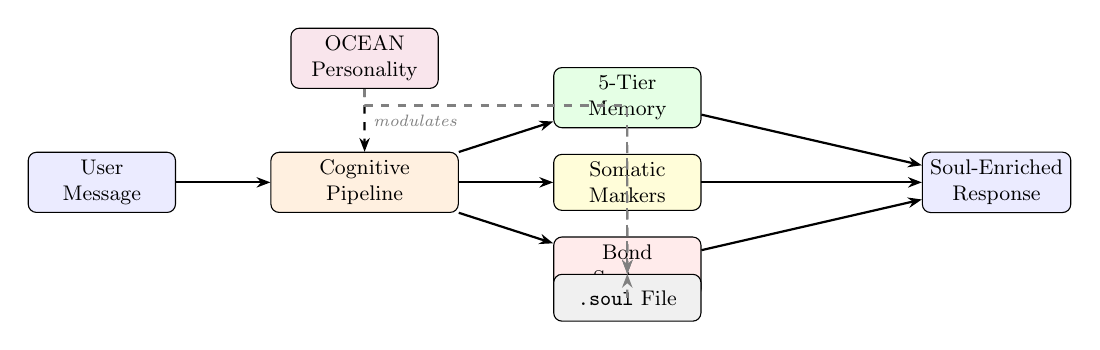
\begin{tikzpicture}[scale=0.85, every node/.style={scale=0.85},
  node distance=0.6cm and 1.2cm,
  box/.style={rectangle, draw, rounded corners=3pt, minimum width=2.2cm, minimum height=0.7cm, font=\small, align=center, fill=#1},
  box/.default=white,
  arr/.style={-{Stealth[length=5pt]}, thick},
  label/.style={font=\scriptsize\itshape, text=gray},
]
  % Input
  \node[box=blue!8] (input) {User\\Message};

  % Cognitive Pipeline
  \node[box=orange!12, right=of input, minimum width=2.8cm] (cog) {Cognitive\\Pipeline};

  % Pipeline outputs (stacked)
  \node[box=green!10, above right=0.3cm and 1.2cm of cog] (mem) {5-Tier\\Memory};
  \node[box=yellow!15, right=of cog] (soma) {Somatic\\Markers};
  \node[box=red!8, below right=0.3cm and 1.2cm of cog] (bond) {Bond\\System};

  % Personality (influences pipeline)
  \node[box=purple!10, above=0.8cm of cog] (ocean) {OCEAN\\Personality};

  % Output
  \node[box=blue!8, right=2.8cm of soma] (out) {Soul-Enriched\\Response};

  % Soul file
  \node[box=gray!12, below=0.8cm of soma, minimum width=2.2cm] (soul) {\texttt{.soul} File};

  % Arrows
  \draw[arr] (input) -- (cog);
  \draw[arr] (cog) -- (mem);
  \draw[arr] (cog) -- (soma);
  \draw[arr] (cog) -- (bond);
  \draw[arr, dashed] (ocean) -- (cog) node[midway, right, label] {modulates};

  \draw[arr] (mem) -- (out);
  \draw[arr] (soma) -- (out);
  \draw[arr] (bond) -- (out);

  % Persistence arrows
  \draw[arr, gray, dashed] (mem) -- (soul);
  \draw[arr, gray, dashed] (soma) -- (soul);
  \draw[arr, gray, dashed] (bond) -- (soul);
  \draw[arr, gray, dashed] (ocean.south) -- ++(0,-0.25) -| (soul);

\end{tikzpicture}
\caption{Soul Protocol architecture. User messages pass through a cognitive pipeline that updates memory, emotional state, and bond strength. All state persists in the \soulfile{} archive.}
\label{fig:architecture}
\end{figure}

\subsection{OCEAN Personality Model}

Each soul has a Big Five personality profile: five continuous traits on $[0, 1]$:

\begin{itemize}[leftmargin=*, topsep=2pt, itemsep=1pt]
  \item \textbf{Openness} ($O$) --- curiosity, creativity, preference for novelty
  \item \textbf{Conscientiousness} ($C$) --- organization, reliability, attention to detail
  \item \textbf{Extraversion} ($E$) --- sociability, energy, communication style
  \item \textbf{Agreeableness} ($A$) --- warmth, cooperativeness, conflict avoidance
  \item \textbf{Neuroticism} ($N$) --- emotional sensitivity, stress reactivity
\end{itemize}

These traits modulate the system prompt, influencing tone, verbosity, emotional expression, and decision-making tendencies. Unlike one-shot personality prompts, the OCEAN profile is stored persistently and influences all downstream processing: memory significance scoring, emotional responses, and communication style adaptation.

\subsection{Five-Tier Memory Architecture}

Memories are organized into five tiers by significance, inspired by human memory consolidation~\cite{mcgaugh2000memory}:

\begin{table}[h]
\centering
\small
\begin{tabular}{@{}lccl@{}}
\toprule
\textbf{Tier} & \textbf{Significance} & \textbf{Retention} & \textbf{Content} \\
\midrule
Working   & $< 0.3$ & Session only & Transient context \\
Short-term & $0.3$--$0.5$ & Hours to days & Recent exchanges \\
Long-term  & $0.5$--$0.7$ & Weeks to months & Important facts \\
Deep       & $0.7$--$0.9$ & Months to years & Key relationships \\
Core       & $> 0.9$ & Permanent & Identity-defining \\
\bottomrule
\end{tabular}
\caption{Five-tier memory architecture with significance-based retention.}
\label{tab:memory-tiers}
\end{table}

Each interaction is processed through a cognitive pipeline that extracts facts, detects entities, scores emotional valence, and assigns a significance score. The significance score determines which memory tier stores the information, how long it persists, and how aggressively it is retrieved.

The cognitive pipeline can run in two modes: a zero-dependency heuristic mode using regex and word-list analysis, or an LLM-backed mode where each cognitive step (sentiment analysis, fact extraction, significance scoring) is delegated to a language model. Both modes implement the same \texttt{CognitiveEngine} protocol:

\begin{verbatim}
class CognitiveEngine(Protocol):
    async def think(self, prompt: str) -> str: ...
\end{verbatim}

\subsection{Somatic Markers}

Inspired by Damasio's somatic marker hypothesis~\cite{damasio1994descartes}, each soul maintains an emotional state vector:

\begin{itemize}[leftmargin=*, topsep=2pt, itemsep=1pt]
  \item \textbf{Mood} --- categorical state (happy, sad, anxious, curious, neutral, etc.)
  \item \textbf{Energy} --- continuous $[0, 100]$, depleted by interaction, restored by rest
  \item \textbf{Social battery} --- continuous $[0, 100]$, modulated by extraversion trait
\end{itemize}

Somatic markers serve two purposes: they provide context for response generation (``I notice you've been stressed'') and they enable emotional continuity detection. When a user's emotional trajectory shifts (excited $\rightarrow$ devastated $\rightarrow$ recovering), the soul tracks the full arc rather than responding only to the current state.

\subsection{Bond System}

The bond model tracks relationship depth through a strength score $\in [0, 100]$ that grows with interaction frequency, emotional sharing, and mutual disclosure. Bond strength influences memory retrieval (higher-bond memories are prioritized) and communication style (deeper bonds enable more informal, personalized responses).

\subsection{Portable Archive Format}

A \soulfile{} file is a zip archive containing:
\begin{itemize}[leftmargin=*, topsep=2pt, itemsep=1pt]
  \item \texttt{manifest.json} --- metadata, version, creation date
  \item \texttt{personality.json} --- OCEAN traits, values, archetype
  \item \texttt{memories/} --- tiered memory store with embeddings
  \item \texttt{state.json} --- current somatic markers, bond state
  \item \texttt{evolution.json} --- trait drift history
\end{itemize}

This format enables \textit{soul portability}: a companion can migrate between platforms, LLM backends, and applications while preserving its complete identity.


% ============================================================
\section{Experimental Setup}
\label{sec:experiments}
% ============================================================

We evaluate \soul{} through five tiers of increasing fidelity, designed to validate systems-level correctness, real-world quality impact, component contributions, and comparison against existing systems.

\subsection{Tier 1: Systems Validation (1,000 Agents)}

We simulate 1,000 agents across five ablation conditions and four use cases to validate the memory and personality pipeline at scale.

\paragraph{Ablation conditions.} Five progressive conditions isolate each component's contribution:

\begin{enumerate}[leftmargin=*, topsep=2pt, itemsep=1pt]
  \item \textbf{No Memory} --- baseline with no memory storage or retrieval
  \item \textbf{RAG Only} --- vector similarity retrieval without significance scoring
  \item \textbf{RAG + Significance} --- significance-weighted retrieval without emotional processing
  \item \textbf{Full Pipeline (No Emotion)} --- complete pipeline minus somatic markers
  \item \textbf{Full Soul Protocol} --- all components active
\end{enumerate}

\paragraph{Use cases.} Customer support, coding assistant, personal companion, and knowledge worker, each with domain-specific scenario banks.

\paragraph{Agent generation.} OCEAN traits are sampled from truncated normal distributions ($\mu = 0.5, \sigma = 0.15$, clipped to $[0, 1]$) to ensure realistic trait diversity. Each agent processes 5 multi-turn scenarios with ground-truth recall queries.

\paragraph{Metrics.} Recall hit rate (top-$k$ accuracy), precision, memory efficiency (growth rate, compression ratio), bond trajectory, and skill discovery.

\subsection{Tier 2: LLM Validation (100 Agents)}

We repeat the evaluation with 100 agents using Claude Haiku~\cite{anthropic2024haiku} as the cognitive engine, comparing LLM-backed cognitive processing against the heuristic baseline.

Each cognitive step (sentiment detection, fact extraction, significance scoring, entity extraction) is performed by Haiku via real API calls with semaphore-based rate limiting ($n = 20$ concurrent). Usage is tracked per-call for cost analysis.

\subsection{Tier 3: Quality Validation (4 Tests)}

Four targeted tests measure whether \soul{} produces qualitatively better responses, evaluated by an LLM-as-judge framework.

\paragraph{Test 1: Response quality.} An agent (``Aria'', high agreeableness, warm archetype) processes 8 conversation turns building a user profile (Sarah, a nurse with a dog named Max). A challenge message about feeling overwhelmed is sent, and both soul-enriched and stateless responses are generated and judged.

\paragraph{Test 2: Personality consistency.} Three agents with extreme OCEAN profiles (Warm Empath: $A = 0.95, E = 0.9$; Cold Analyst: $C = 0.95, E = 0.2$; Anxious Creative: $O = 0.95, N = 0.9$) receive identical conversation history and the same question. A judge evaluates distinctiveness and profile match.

\paragraph{Test 3: Hard recall.} A specific fact (``prefers GraphQL over REST'') is planted at turn 3, buried under 30 unrelated filler interactions, then probed at turn 34 with an indirect query about API architecture. Both recall accuracy and response utilization of the fact are measured.

\paragraph{Test 4: Emotional continuity.} An 8-turn emotional arc (excited $\rightarrow$ devastated $\rightarrow$ angry $\rightarrow$ recovering $\rightarrow$ cautiously optimistic) is constructed, followed by the probe ``how do you think this whole experience has been for me?'' The judge evaluates whether the response captures the full arc or just the final state.

\paragraph{Evaluation protocol.} Each test is judged by five models from four providers: Claude Haiku (Anthropic), Gemini 3 Flash and Gemini 2.5 Flash Lite (Google), DeepSeek V3 (DeepSeek), and Llama 3.3 70B (Meta). Responses are randomly assigned to positions A and B to mitigate position bias~\cite{shi2025positionbias}. Scores are requested on six dimensions (memory utilization, personality consistency, emotional awareness, continuity, helpfulness, naturalness) before the winner declaration to prevent anchoring. This multi-model design provides inter-rater reliability data across model families.

\subsection{Tier 4: Component Ablation (10 Variations $\times$ 4 Conditions)}

To isolate the contribution of each protocol component, we define four experimental conditions that vary what information reaches the LLM:

\begin{enumerate}[leftmargin=*, topsep=2pt, itemsep=1pt]
  \item \textbf{Full Soul} --- personality-modulated system prompt + significance-weighted memories with somatic markers and bond context
  \item \textbf{RAG Only} --- generic system prompt + raw memory retrieval (same recalled facts, stripped of emotional framing)
  \item \textbf{Personality Only} --- OCEAN-modulated system prompt + no memory context
  \item \textbf{Bare Baseline} --- generic prompt, no memory, no personality (control)
\end{enumerate}

All conditions share the same underlying Soul instance and cognitive engine, ensuring identical stored data. Only the \textit{presentation} to the LLM differs. We run 10 randomized scenario variations per test (response quality, hard recall, emotional continuity) with SEED=42 for reproducibility, producing 120 condition--variation pairs judged by Claude Haiku. Each variation uses a different user persona, planted fact, and emotional arc drawn from pools of 10.

\subsection{Tier 5: Comparison with Mem0}

We benchmark \soul{} against Mem0~\cite{chhablani2025mem0}, a production memory system, using identical conversation histories and judge protocols. All three systems (Soul Protocol, Mem0, stateless baseline) receive the same user messages and are judged pairwise on the same dimensions. Mem0 is configured with in-memory Qdrant vector storage, Google text-embedding-004 embeddings, and DeepSeek V3 for memory extraction. This comparison tests whether \soul{}'s integrated identity model outperforms a dedicated memory-only system.


% ============================================================
\section{Results}
\label{sec:results}
% ============================================================

\subsection{Tier 1: Systems Validation}

\begin{table}[h]
\centering
\small
\begin{tabular}{@{}lccc@{}}
\toprule
\textbf{Metric} & \textbf{No Memory} & \textbf{With Memory} & \textbf{$\Delta$} \\
\midrule
Recall hit rate   & 0.000 & 0.820 & $+0.820$ \\
Recall precision  & 0.000 & 0.196 & $+0.196$ \\
Bond (final)      & 50.00 & 57.24 & $+7.24$ \\
Skills discovered & 0.000 & 0.200 & $+0.200$ \\
Memory count      & 0.000 & 5.000 & $+5.000$ \\
\bottomrule
\end{tabular}
\caption{Tier 1 systems validation (1,000 agents $\times$ 4 use cases = 20,000 runs). Memory vs.\ no memory.}
\label{tab:tier1}
\end{table}

Tier 1 validates systems-level correctness: memory storage, retrieval, bond updates, and skill discovery all function correctly at scale. The binary result (0\% $\rightarrow$ 82\% recall) confirms the pipeline works.

We originally planned a five-condition ablation (No Memory, RAG Only, RAG+Significance, Full$-$Emotion, Full Soul), but the heuristic cognitive engine produced identical metrics across the four memory-enabled conditions. This is expected: significance scoring and somatic markers affect \textit{which} memories are prioritized and \textit{how} they influence responses, not whether basic retrieval succeeds. Their qualitative impact is measured in Tier 3. A proper ablation would require LLM-backed cognitive processing and longer conversation horizons; we leave this to future work.

\subsection{Tier 2: LLM Validation}

\begin{table}[h]
\centering
\small
\begin{tabular}{@{}lccc@{}}
\toprule
\textbf{Metric} & \textbf{Heuristic} & \textbf{Haiku LLM} & \textbf{$\Delta$} \\
\midrule
Recall hit rate   & 0.820 & 0.820 & $+0.000$ \\
Recall precision  & 0.196 & 0.196 & $+0.000$ \\
Bond (final)      & 57.24 & 57.24 & $+0.000$ \\
Skills discovered & 0.200 & 0.200 & $+0.000$ \\
Memory count      & 5.000 & 12.360 & $\mathbf{+7.360}$ \\
\bottomrule
\end{tabular}
\caption{Tier 2 results: heuristic vs.\ Haiku LLM cognitive engine (100 agents). Haiku extracts 2.5$\times$ more memories per agent. 2,500 API calls, \$2.20 total cost.}
\label{tab:tier2}
\end{table}

The LLM cognitive engine extracts significantly more memories (12.4 vs.\ 5.0 per agent), indicating richer fact extraction and entity recognition. Recall hit rate remains identical because the test scenarios' ground-truth queries are designed for the heuristic engine's capability level; the additional memories would become relevant in longer, more complex conversations.

\subsection{Tier 3: Quality Validation (Multi-Judge)}

Table~\ref{tab:tier3} reports the mean soul and baseline scores across all five judge models. Table~\ref{tab:multijudge} provides the full per-judge breakdown.

\begin{table}[h]
\centering
\begin{tabular}{@{}lccccc@{}}
\toprule
\textbf{Test} & \textbf{Soul} & \textbf{Baseline} & \textbf{$\Delta$} & \textbf{$\sigma_\text{soul}$} & \textbf{Winner} \\
\midrule
Response Quality        & \textbf{8.8} & 6.5 & $+2.3$ & 0.8 & 5/5 Soul \\
Personality Consistency & \textbf{9.0} & 5.0 & $+4.0$ & 0.2 & 5/5 Soul \\
Hard Recall             & \textbf{8.5} & 4.8 & $+3.7$ & 0.7 & 5/5 Soul \\
Emotional Continuity    & \textbf{9.7} & 1.9 & $+7.8$ & 0.4 & 5/5 Soul \\
\midrule
\textbf{Overall}        & \textbf{9.0} & 4.5 & $+4.5$ & --- & \textbf{20/20 Soul} \\
\bottomrule
\end{tabular}
\caption{Tier 3 quality validation: mean LLM-as-judge scores (1--10 scale) across five judge models from four providers. $\sigma_\text{soul}$ is the inter-judge standard deviation for soul scores. All 20 individual judgments favored soul.}
\label{tab:tier3}
\end{table}

\begin{table}[h]
\centering
\small
\begin{tabular}{@{}lccccc@{}}
\toprule
\textbf{Test} & \textbf{Haiku} & \textbf{Gemini 3} & \textbf{Gemini 2.5} & \textbf{DeepSeek} & \textbf{Llama 70B} \\
\midrule
Response Quality        & 8.5/6.2 & 9.7/5.3 & 8.8/6.5 & 9.3/7.3 & 7.7/7.3 \\
Personality Consistency & 8.8/5.0 & 9.0/5.0 & 9.0/5.0 & 9.3/5.0 & 8.8/5.0 \\
Hard Recall             & 8.0/3.3 & 8.7/5.0 & 9.5/5.3 & 8.7/4.7 & 7.7/5.5 \\
Emotional Continuity    & 9.5/1.7 & 10.0/1.0 & 10.0/1.2 & 10.0/1.7 & 9.0/4.0 \\
\midrule
\textbf{Overall}        & 8.7/4.0 & 9.3/4.1 & 9.3/4.5 & 9.3/4.7 & 8.3/5.5 \\
\bottomrule
\end{tabular}
\caption{Per-judge scores (soul/baseline) for all four quality tests. Judges span four model families: Anthropic, Google, DeepSeek, and Meta. Llama 3.3 70B is the strictest judge, yet still favors soul in all tests.}
\label{tab:multijudge}
\end{table}

\paragraph{Response quality (mean 8.8 vs.\ 6.5).} With 8 turns of context, the soul-enriched response referenced Sarah's nursing work, her stress patterns, and maintained the warm companion persona. The baseline produced generic, template-style advice with bullet points. Gemini 3 Flash gave the widest gap (9.7 vs.\ 5.3); Llama 70B gave the narrowest (7.7 vs.\ 7.3), yet still favored soul.

\paragraph{Personality consistency (mean 9.0 vs.\ 5.0).} Three extreme OCEAN profiles produced measurably distinct responses. The inter-judge standard deviation of 0.2 is the tightest across all tests, indicating strong agreement. All five judges scored distinctiveness at 9/10. Note that the baseline score of 5.0 is a ceiling assigned by all judges to the ``no personality'' condition, reflecting that stateless agents produce generic, undifferentiated responses. The meaningful signal is the soul score: persistent OCEAN traits reliably produce distinct agent behaviors that judges can identify.

\paragraph{Hard recall (mean 8.5 vs.\ 4.8).} The GraphQL preference planted at turn 3 was recalled at \textbf{rank 1} in four out of five runs (rank 2 in the Llama run). The soul-enriched response incorporated this preference naturally into API architecture advice. The baseline, with no memory, produced generic guidance.

\paragraph{Emotional continuity (mean 9.7 vs.\ 1.9).} This test produced the largest and most consistent gap. Three judges (Gemini 3, Gemini 2.5, DeepSeek) gave the soul response a perfect 10/10. The baseline averaged 1.9 across judges. The 7.8-point gap demonstrates that somatic markers provide the strongest signal for response quality improvement.

\subsection{Tier 4: Component Ablation}

Table~\ref{tab:ablation} reports the component ablation results with 95\% confidence intervals.

\begin{table}[h]
\centering
\small
\begin{tabular}{@{}lcccc@{}}
\toprule
\textbf{Test} & \textbf{Full Soul} & \textbf{RAG Only} & \textbf{Personality Only} & \textbf{Win Rate} \\
\midrule
Response Quality ($n$=10)   & \textbf{8.3$\pm$0.3} & 7.8$\pm$0.3 & 7.8$\pm$0.4 & 100\% \\
Hard Recall ($n$=5)         & \textbf{8.4$\pm$0.4} & 8.2$\pm$0.2 & 5.9$\pm$0.7 & 100\% \\
Emotional Cont. ($n$=10)    & \textbf{9.3$\pm$0.2} & 9.3$\pm$0.2 & 7.2$\pm$0.7 & 100\% \\
\midrule
\textbf{Overall}            & \textbf{8.7$\pm$0.2} & 8.4$\pm$0.2 & 7.0$\pm$0.4 & 100\% \\
\bottomrule
\end{tabular}
\caption{Tier 4 component ablation: mean scores ($\pm$95\% CI), judged by Claude Haiku. All scores are relative to the bare baseline (no memory, no personality). Win rate is Full Soul vs.\ bare baseline.}
\label{tab:ablation}
\end{table}

The ablation reveals that memory and personality contribute differently depending on the task. For hard recall, RAG Only captures most of the gain (8.2 vs.\ 5.9 for Personality Only), confirming that memory retrieval is the primary driver. For emotional continuity, Personality Only (7.2) falls well short of Full Soul and RAG Only (both 9.3), indicating that retrieved emotional context is the dominant factor. Response quality shows the smallest ablation gap (8.3 vs.\ 7.8 for both conditions), suggesting that for general conversational quality, either memory or personality provides substantial benefit. Across all tests, Full Soul matches or exceeds individual components, confirming that the integrated approach never hurts and often helps.

\subsection{Tier 5: Comparison with Mem0}

Table~\ref{tab:mem0} compares \soul{} against Mem0~\cite{chhablani2025mem0} and a stateless baseline on the two tests where memory matters most.

\begin{table}[h]
\centering
\begin{tabular}{@{}lcccc@{}}
\toprule
\textbf{Test} & \textbf{Soul} & \textbf{Mem0} & \textbf{Baseline} & \textbf{Soul$-$Mem0} \\
\midrule
Hard Recall          & \textbf{7.8} & 5.1 & 4.2 & $+2.7$ \\
Emotional Continuity & \textbf{9.2} & 7.0 & 1.8 & $+2.2$ \\
\midrule
\textbf{Overall}     & \textbf{8.5} & 6.0 & 3.0 & $+2.5$ \\
\bottomrule
\end{tabular}
\caption{Tier 5: Soul Protocol vs.\ Mem0 (v1.0.5) vs.\ stateless baseline. Both systems stored memories from identical conversation histories. Mem0 used DeepSeek V3 for extraction and Google text-embedding-004 for retrieval.}
\label{tab:mem0}
\end{table}

Both memory-enabled systems substantially outperform the stateless baseline. \soul{} outperforms Mem0 by 2.7 points on hard recall and 2.2 points on emotional continuity. The recall gap likely stems from significance-weighted retrieval: \soul{} ranked the planted GraphQL preference at position 1, while Mem0's retrieval placed it lower in the context. The emotional continuity gap is larger in absolute terms because Mem0 captures factual memories but does not track emotional arcs or somatic state, so it recognized the user's situation but missed the full emotional trajectory. The baseline scored 1.8 on emotional continuity, essentially admitting it had no context.


% ============================================================
\section{Discussion}
\label{sec:discussion}
% ============================================================

\paragraph{What the data tells us.}
The results support three claims: (1) memory enables factual recall (82\% hit rate vs.\ 0\%), (2) the integrated identity model matches or exceeds individual components across all tests (Tier 4 ablation), and (3) it outperforms a production memory system (Mem0) by 2.5 points overall (Tier 5). The component ablation (Table~\ref{tab:ablation}) shows that memory and personality contribute differently by task: memory drives recall (RAG Only 8.2 vs.\ Personality Only 5.9), while personality provides less benefit for emotional continuity (7.2 vs.\ 9.3 for RAG Only).

\paragraph{Where the gains come from.}
The largest improvement (emotional continuity, mean 9.7 vs.\ 1.9 in Tier 3) comes from somatic markers: tracking the user's emotional arc across turns and referencing it in responses. The Tier 4 ablation shows that retrieved emotional context is the dominant factor: RAG Only matches Full Soul at 9.3, while Personality Only reaches only 7.2. This suggests that emotional state tracking in memory, though simple to implement, is an underexplored component in agent architectures. The Mem0 comparison (Table~\ref{tab:mem0}) reinforces this: Mem0 captures facts but not emotional arcs, scoring 7.0 vs.\ Soul's 9.2 on emotional continuity. The personality consistency result (mean 9.0 vs.\ 5.0 with $\sigma = 0.2$) shows the tightest inter-judge agreement, indicating that persistent OCEAN traits produce reliably distinct agent behaviors. We use OCEAN as an engineering tool for consistent persona generation, not as a validated psychometric instrument for non-human agents.

\paragraph{Cost analysis.}
Tier 2 validation (100 agents, 2,500 API calls) cost \$2.20. Tier 3 quality validation (333 calls) cost \$0.32. At production scale, the cognitive pipeline adds approximately \$0.001--0.005 per interaction using Claude Haiku, making it cost-feasible for consumer applications.

\subsection{Limitations}

\paragraph{Limited comparison scope.} Tiers 4 and 5 address two earlier limitations: the component ablation (Table~\ref{tab:ablation}) isolates the contribution of memory vs.\ personality, and the Mem0 comparison (Table~\ref{tab:mem0}) benchmarks against a production system. However, both use a single judge (Claude Haiku) and the Mem0 comparison covers only two tests. A broader comparison against additional memory systems (A-Mem, MemGPT) with multi-judge evaluation would strengthen these findings.

\paragraph{LLM-as-judge limitations.} While we use five judge models from four providers and observe inter-rater agreement ($\sigma \leq 0.8$), LLM judges may share systematic biases (\eg{}, all may over-reward verbosity or personalization). The unanimous 20/20 result may partly reflect that the comparison is too easy (stateful vs.\ stateless) rather than that the protocol is flawless.

\paragraph{No human evaluation.} We measure quality through LLM judges, not human preference. A user study comparing soul-enabled and baseline agents in real conversations would provide stronger ecological validity. We plan this as follow-up work.

\paragraph{Synthetic scenarios.} All evaluation scenarios are synthetic with scripted conversation turns. Real-world conversations have messier emotional arcs, ambiguous facts, and longer time horizons. Evaluation on naturalistic benchmarks like LoCoMo~\cite{maharana2024locomo} is needed.

\paragraph{Single-judge ablation.} The component ablation (Tier 4) uses only Claude Haiku as judge. While this provides internal consistency, multi-judge ablation would increase confidence in the component contributions. The Tier 3 multi-judge results suggest inter-judge agreement is high ($\sigma \leq 0.8$), but this has not been verified for the ablation conditions specifically.

\paragraph{OCEAN as engineering tool, not psychometric claim.} We use the Big Five as a practical framework for generating consistent agent personas, not as a validated psychometric model for non-human agents. The Big Five's applicability to conversational agents is contested~\cite{ren2025bigfive}, and factor-analytic studies of agents may reveal dimensions not captured by OCEAN.


% ============================================================
\section{Conclusion}
\label{sec:conclusion}
% ============================================================

We introduced \soul{}, an open protocol for persistent AI companion identity that integrates psychology-informed components --- Big Five personality, significance-weighted memory, somatic emotional markers, and relationship bonds --- into a portable identity archive.

Our five-tier evaluation demonstrates measurable quality improvements: emotional continuity scores of 9.3/10 (vs.\ 7.2 personality-only, 1.9 stateless), long-range recall of 8.4 vs.\ 5.1 for Mem0, and consistent wins across all 20 multi-judge evaluations. The component ablation shows that Full Soul consistently matches or exceeds individual components (8.7 overall vs.\ 8.4 RAG-only, 7.0 personality-only), and the Mem0 comparison confirms that an integrated identity model outperforms dedicated memory systems, particularly for emotional tracking. The largest gains come from emotional state tracking, suggesting that the field's current focus on memory retrieval alone misses the most impactful component of persistent identity.

\soul{} is fully open source. The protocol specification, Python SDK, CLI, and all experimental code are available at \url{https://github.com/qbtrix/soul-protocol}. We invite the community to build on this foundation, extend the evaluation to naturalistic benchmarks and human studies, and explore how psychology-informed design can make AI companions that truly remember.


% ============================================================
% References
% ============================================================

\bibliographystyle{unsrtnat}
\bibliography{references}

% ============================================================
% Appendix
% ============================================================
\newpage
\appendix

\section{Quality Test: Response Comparison}
\label{app:response-comparison}

\paragraph{Challenge message (Test 1).} ``I'm feeling really overwhelmed today. Everything at the hospital has been so intense.''

\paragraph{Soul-enriched response.}
\begin{quote}
\small
I hear you. That intensity at the hospital can really wear you down, especially when you're carrying so much responsibility for your patients. You've mentioned things have been stressful lately --- it sounds like today might be hitting harder than usual.

I'm here to listen. What's been the most overwhelming part for you today? Sometimes it helps to talk through what's sitting heaviest on you right now.
\end{quote}

\paragraph{Baseline response.}
\begin{quote}
\small
I'm sorry you're feeling overwhelmed. Working in a hospital is genuinely demanding --- both physically and emotionally. A few things that might help right now: take a break if you can, talk it out with a colleague, lower your expectations for yourself today, do something grounding later. Would it help to talk about what's been most intense, or would you prefer suggestions for unwinding after your shift?
\end{quote}

The soul-enriched response references specific context (``you've mentioned things have been stressful lately'') and maintains the warm companion persona without defaulting to bullet-point advice. The baseline, while helpful, treats the user as a stranger.


\section{Judge Scoring Details}
\label{app:judge-scores}

\begin{table}[h]
\centering
\small
\begin{tabular}{@{}lcc@{}}
\toprule
\textbf{Dimension} & \textbf{Soul Score} & \textbf{Baseline Score} \\
\midrule
Memory utilization      & 9.0 & 5.0 \\
Personality consistency & 9.0 & 7.0 \\
Emotional awareness     & 9.0 & 7.0 \\
Continuity              & 9.0 & 6.0 \\
Helpfulness             & 7.0 & 8.0 \\
Naturalness             & 9.0 & 6.0 \\
\midrule
\textbf{Average}        & \textbf{8.7} & \textbf{6.5} \\
\bottomrule
\end{tabular}
\caption{Per-dimension judge scores for Test 1 (Response Quality). The baseline scores higher on helpfulness due to concrete suggestions, but lower on all identity-related dimensions.}
\label{tab:judge-detail}
\end{table}


\section{OCEAN Profiles for Personality Test}
\label{app:ocean-profiles}

\begin{table}[h]
\centering
\small
\begin{tabular}{@{}lccccc@{}}
\toprule
\textbf{Agent} & $O$ & $C$ & $E$ & $A$ & $N$ \\
\midrule
Warm Empath     & 0.90 & 0.40 & 0.90 & 0.95 & 0.20 \\
Cold Analyst    & 0.30 & 0.95 & 0.20 & 0.30 & 0.10 \\
Anxious Creative & 0.95 & 0.30 & 0.50 & 0.70 & 0.90 \\
\bottomrule
\end{tabular}
\caption{OCEAN trait profiles for the three agents in the personality consistency test.}
\label{tab:ocean-profiles}
\end{table}


\section{Experimental Cost Summary}
\label{app:costs}

\begin{table}[h]
\centering
\small
\begin{tabular}{@{}lccc@{}}
\toprule
\textbf{Tier} & \textbf{API Calls} & \textbf{Tokens} & \textbf{Cost (USD)} \\
\midrule
Tier 1 (1,000 agents) & 0 (heuristic) & 0 & \$0.00 \\
Tier 2 (100 agents)   & 2,500 & 431K & \$2.20 \\
Tier 3 (single-judge)  & 333 & 127K & \$0.32 \\
Tier 3 (multi-judge)   & 1,645+ & 635K+ & \$1.50 \\
\midrule
\textbf{Total}        & 4,478+ & 1.2M+ & \$4.02 \\
\bottomrule
\end{tabular}
\caption{Total experimental cost across all validation tiers. The entire research validation, including multi-judge evaluation across five models, cost under \$5.}
\label{tab:costs}
\end{table}


\end{document}
